\documentclass{article}

\usepackage[british]{babel}
\usepackage{cite}
\usepackage{graphicx}
\usepackage{url}
\usepackage{afterpage}
\renewcommand*\ttdefault{txtt}

\usepackage{listings}
\lstset{language=R,basicstyle=\ttfamily}

\title{LLAMA: Leveraging Learning to Automatically Manage Algorithms}

\author{Lars Kotthoff}
\date{}

\begin{document}

\begin{titlepage}

\maketitle
\thispagestyle{empty}

\begin{center}
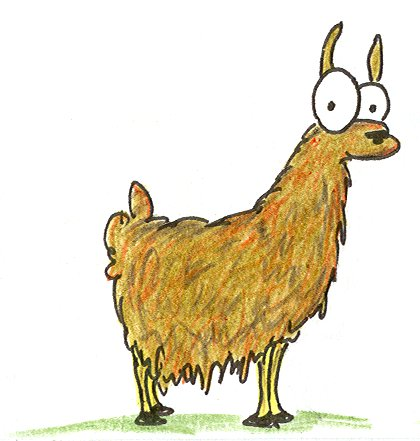
\includegraphics[width=.5\textwidth]{llama.jpg}
\end{center}

\begin{abstract}
Algorithm portfolio and selection approaches have achieved remarkable
improvements over single solvers. However, the implementation of such systems is
often highly customised and specific to the problem domain. This makes it
difficult for researchers to explore different techniques for their specific
problems. We present LLAMA, a modular and extensible toolkit implemented as an R
package that facilitates the exploration of a range of different portfolio
techniques on any problem domain. It implements the algorithm selection
approaches most commonly used in the literature and leverages the extensive
library of machine learning algorithms and techniques in R. We describe the
current capabilities and limitations of the toolkit and illustrate its usage on
a set of example SAT problems.
\end{abstract}

\vspace*{\stretch{1}}

\begin{center}
This document corresponds to LLAMA version 0.9.1.
\end{center}

\end{titlepage}


\renewenvironment{knitrout}{\setlength{\topsep}{0mm}}{}


\section*{Quick start}

So you know about algorithm portfolios and selection and just want to get
started. Here we go. In your R shell, type

\begin{knitrout}
\definecolor{shadecolor}{rgb}{0.969, 0.969, 0.969}\color{fgcolor}\begin{kframe}
\begin{alltt}
\hlkwd{install.packages}\hldef{(}\hlsng{"llama"}\hldef{)}
\hlkwd{library}\hldef{(llama)}
\end{alltt}
\end{kframe}
\end{knitrout}

to install and load LLAMA. We're going to assume that you have two input CSV
files for your data -- features and times. The rows designate problem instances
and the columns feature and solver names. All files must have an 'ID' column
that allows to link them. Load them into the data structure required by LLAMA as
follows.

\begin{knitrout}
\definecolor{shadecolor}{rgb}{0.969, 0.969, 0.969}\color{fgcolor}\begin{kframe}
\begin{alltt}
\hldef{data} \hlkwb{=} \hlkwd{input}\hldef{(}\hlkwd{read.csv}\hldef{(}\hlsng{"features.csv"}\hldef{),} \hlkwd{read.csv}\hldef{(}\hlsng{"times.csv"}\hldef{))}
\end{alltt}
\end{kframe}
\end{knitrout}

You can also use the SAT solver data that comes with LLAMA by running

\begin{knitrout}
\definecolor{shadecolor}{rgb}{0.969, 0.969, 0.969}\color{fgcolor}\begin{kframe}
\begin{alltt}
\hlkwd{data}\hldef{(satsolvers)}
\hldef{data} \hlkwb{=} \hldef{satsolvers}
\end{alltt}
\end{kframe}
\end{knitrout}

Now partition the entire set of instances into training and test sets for
cross-validation.

\begin{knitrout}
\definecolor{shadecolor}{rgb}{0.969, 0.969, 0.969}\color{fgcolor}\begin{kframe}
\begin{alltt}
\hldef{folds} \hlkwb{=} \hlkwd{cvFolds}\hldef{(data)}
\end{alltt}
\end{kframe}
\end{knitrout}

This will give you 10 folds for cross-validation. Now we're ready to train
our first model. To do that, we'll need some machine learning algorithms --
we're going to use a random forest classifier. Now train a simple classification
model that predicts the best algorithm.































































































